\SetKw{State}{state}
\SetKw{Send}{send}
\SetKw{Wait}{wait}
\SetKw{Call}{call}
\SetKw{Return}{return}

\SetKwComment{Comment}{//}{}

\SetKwProg{Function}{function}{}{end}

\SetKwBlock{parallelblk}{Do In Parallel}{end}
\SetKwBlock{atomicblk}{atomic}{end}

\SetKwFunction{atomicAdd}{AtomicAdd}
\SetKwFunction{sortps}{sortByPredecessorSize}
\SetKwFunction{clientSubmit}{Client::SubmitOp}
\SetKwFunction{clientWait}{Client::WaitOp}
\SetKwFunction{leaderSubmit}{Leader::SubmitOpRecv}
\SetKwFunction{replicaCoord}{Replica::coordRequestRecv}
\SetKwFunction{shardMain}{Leader::shardMain}
\SetKwFunction{CR}{Leader::CoordinationRequest}
\SetKwFunction{CRReply}{Leader::CoordinationResponse}
\SetKwFunction{append}{.append}
\SetKwFunction{find}{.find}
\SetKwFunction{popO}{.popOrderedAndStale()}

\algnewcommand{\IfThenElse}[3]{% \IfThenElse{<if>}{<then>}{<else>}
  \algorithmicif\ #1\ \algorithmicthen\ #2\ \algorithmicelse\ #3}

\algnewcommand{\IfThen}[2]{% \IfThenElse{<if>}{<then>}{<else>}
  \algorithmicif\ #1\ \algorithmicthen\ #2}

\section{\sys{}}
\label{sec:design}
% 1. what are the key features it needs to do. which component of the protocol does that.
% 2. include parts in the motivation that describe why you can't simply do "X". and then in design you can refer to motivation...

\sys{} achieves two competing goals: First, it guarantees \multidispatch{}
linearizability, even in the face of concurrent requests both within
and across clients that span multiple shards. Second, it offers lower
end-to-end application compared to a similar Linearizable system.

% Design V1: Clients issue multiple ops and send coordination requests to prior ops
% (as in our protocol). Ops are buffered at shard leaders until they are "coordinated."
% The first op in a sequence is trivially coordinated. Once coordinated, an op is
% replicated to a quorum, and then sends a coordination message to next op in sequence.
% Problem: e2e = N * QRT + (N-1) * RTT/2
% Solution: Decouple fault-tolerance from ordering.

To do so, \sys{} employs three techniques: First, to satisfy \MDL{}'s
suffix-complete failure semantics, \sys{} clients orchestrate coordination
between its operations. More specifically, this coordination ensures
an operation's predecessor commits (and is thus fault-tolerant) before
the operation itself commits.

% Design V2: Divide log into epochs. Replicate ops in current epoch immediately and allow
% them to send coordination responses. This preserves failure semantics because op is now
% fault-tolerant.
% Feature: improved e2e = 2? * QRT + (N-1) * RTT/2 + E
% Problem: Ops within epoch may not respect issue order across clients.
% Solution: Propagate Lamport timestamps and sort ops in epoch by timestamps.

As discussed in Section~\ref{fig:concurrentbatches}, naively allowing
a client's operations to be ordered separately at multiple shards can lead
to violations of \MDL{}'s invocation-order guarantees. But many existing
state-machine replication protocols, including Raft, couple fault-tolerance
and ordering. Thus, it would seem that to guarantee both per-client issue order
and suffix-complete failure semantics, each operation must wait to replicate
until after its predecessor finishes replicating (and thus being ordered).
Unfortunately, the end-to-end latency of an application issuing $N$ operations
to such a system would be approximately $N$ times one quorum round-trip plus
one inter-shard message. This is worse than linearizable Raft, which just requires
one quorum round-trip per operation.

To offer lower end-to-end application latency, \sys{} thus decouples
fault-tolerance from ordering by dividing each shard's log into \textit{epochs}.
An operation is first replicated as part of a \textit{pending operation set},
after which it can notify its successor. This replication can proceed in
parallel for all operations in a client's sequence. At the end of each epoch,
the operations in the pending operation set are ordered by placing them into
the shard's log, requiring a second quorum round trip.     

% Design V3: Our full protocol.

Finally, to ensure per-client issue order is respected both within and across
shard epochs, \sys{} assigns each operation a Lamport timestamp and sorts each
epoch's operations by their timestamps. Upon arrival at a shard, an operation
is assigned an initial, tentative timestamp based on the maximum of the timestamps of
all operations that have been replicated and coordinated previously at the shard.
Operations then propagate these timestamps to the successors in their coordination
messages, and successors update their timestamps to always be greater than their
predecessors.

We now discuss each of these techniques in turn. \sys{}'s full client and shard
protocols are specified in Algorithms~\ref{clientprotocol} and~\ref{shardprotocol}. 

% Jeff: I think this is mostly covered (or will be) in the previous two sections.
% Existing protocols that provide \sdl assume clients abide by the restriction to single-dispatch requests, having at most one outstanding request at a time. This assumption comes from the definition of linearizability, which requires individual clients to behave sequentially. These protocols, such as Paxos, Raft, Viewstamped Replication, Zab, do not provide any guarantees on the order that concurrent requests issued from a single client take effect. Our definition of \md specifies that concurrent requests issued from a single client take effect in invocation order. 

\begin{figure}[!htb]
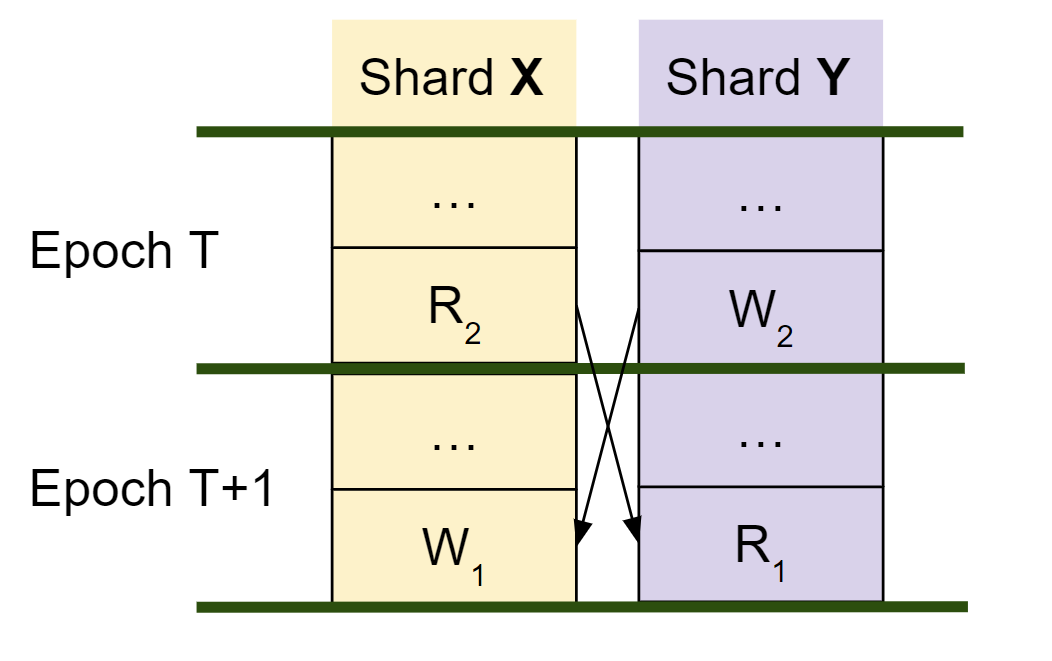
\includegraphics[scale=.3]{sorted_batching_wrong.png}
\caption{Example execution of sorted batching without coordination requirement. This execution leads to an incorrect execution that contains a cycle and is not \mdl. The execution is the same execution as that of figure \ref{fig:concurrentbatches}, but now the second request issued by each client arrives in an earlier epoch. Even if sorted in their respective epochs, they are not ordered across epochs without coordination.}
\label{fig:sortedbatchingwrong}
\end{figure}

% Since all requests can not be known a priori, we make use of epochs at each shard, and guarantee sorted execution order within each epoch, as well as a safe ordering across epochs. With this approach, we can prune request interleavings that might lead to cycles upfront, rather than running cycle detection and subsequently failing execution. While this unnecessarily prevents some subset of safe interleavings, the latter scales poorly for very large cycles.

\subsection{Client-Driven Coordination}

Operations in a multi-shard system can fail independently, e.g., during leader failure at one shard. 
When clients issue multiple operations
concurrently, this also makes it possible for an earlier operation to fail while a later
operation succeeds. But such a case would violate \MDL{}'s suffix-complete failure semantics.  
\sys{} thus introduces client-driven \textit{coordination requests (CR)} between shards to preserve these semantics.

When each client submits an operation to a shard, in parallel it also submits a CR
to the shard of its predecessor operation with the identity of the shard of its successor.
For some operation issued by client $C$
with sequence number $s$, a predecessor operation is defined as the concurrent
operation that client $C$ issued with sequence number $s-1$. If client $C$ does not
have any other outstanding operations, then the operation's predecessor is
\texttt{null}.

An operation is considered \textit{replicated} once it has been acknowledged by a
quorum of replicas. Further, it is considered \textit{coordinated} if the shard has
received a \textit{coordination response} from the shard leader of the operation's predecessor.
(Operations without a predecessor are vacuously coordinated.)
Upon receiving a coordination request, a shard first waits until the operation is
replicated and coordinated and then sends a coordination response to the shard leader
of its successor. This inductively guarantees all of an operation's predecessors will
eventually succeed.

\subsection{Decoupling Fault-Tolerance \& Ordering}

\sys{} decouples fault-tolerance and ordering to allow operations to allows shards to process operations
from the same client in parallel. This is key to \sys{}'s ability to offer lower end-to-end application
latency.

Shards divide their execution into a series of \textit{epochs}. The epoch length is a system parameter,
and epochs need not be synchronized across shards.

Each operation then requires two rounds between a shard leader and a quorum of its replicas.
When the operation arrives at the shard leader, it is replicated first for fault-tolerance
and placed in an unordered pending operation set. As mentioned above, this also allows the shard
leader to respond to a coordination request if the operation has a successor. At the end of the epoch,
the shard leader places all of the operations that have been replicated and coordinated
since the end of the last epoch into its (ordered) log and sends a second message to a quorum of
replicas to commit this order. (We describe how the leader orders requests in more detail in the next
section.)

Operations may fail to be included in the current epoch for one of two reasons:
(1) they may time out while waiting to receive a coordination response from their predecessor,
which we implement by bounding the number of epochs during which it can exist in the pending operation set,
or (2) they may receive an explicit FAIL response for its coordination response. The latter can happen
if, for instance, a leader failure occurred at one of the predecessors' shards.

An operation that has been included in the ordered log at both a leader and a quorum of replicas
is considered \textit{ordered}. Leaders and replicas execute ordered requests in the same fashion
as Raft~\cite{ongaro2014raft}, and leaders respond to clients after executing an operation.

\subsubsection{Operation vs. End-To-End Latency}

Although decoupling fault-tolerance and ordering increases each operation's latency by introducing a
second round of messages between a leader and its replicas, it still improves end-to-end application
latency of applications that issue more than a few operations. This is because shards can replicate
operations from the same client in parallel. Further, they can commit an order and execute operations
in parallel, too. Only the cross-shard coordination messages are sent sequentially for a client's
sequence of operations.

As a result, a client's end-to-end application latency when using \sys{} scales by a factor
of the one-way cross-shard latency as the number of operations increases. In contrast,
the latency of applications using a \singledispatch{} system scales by a factor of the
quorum round-trip latency. Our evaluation in Section~\ref{sec:eval} bears out this claim.

\subsection{Lamport Timestamps For Issue Order}

Need to describe Lamport timestamp assignment and propagation.

A total execution order is guaranteed by ensuring shards sort \textit{ordered} requests by increasing size of predecessor set within each epoch and execute requests in monotonically increasing epoch order. As mentioned before, sorting requests by the number of predecessors ensures a safe total ordering exists. The client library keeps track of the total number of outstanding requests at a given time, which it submits with each request for its predecessor set size. Requests with equal predecessor set sizes are sorted by arrival order to guarantee a stable sort across replicas.

An \textit{ordered} request is one that has been committed and coordinated. \md commits requests with the same mechanism as regular Raft, and it coordinates requests with the use of CR messages sent between shard leaders. Since executing requests now depends on two requirements being fulfilled, commitment as well as coordination, shards keep track of two logs. The first is an execution log containing \textit{ordered} requests that is segmented by epochs, and the second is a buffered log where request entries exist until they are committed (replicated at a majority) and coordinated. While this could be achieved with one log that contains holes and is executed in custom nonlinear order, we choose to break the log into two logs to simplify things and to remain consistent with Raft. We include a final \textit{ordering} inter-replica agreement at the end of each epoch to move requests between logs.

\md can only guarantee a safe total ordering across epochs of shards if it executes \textit{ordered} requests. Figure ~\ref{fig:sortedbatchingwrong} shows an execution that does not abide by this constraint, and only sorts committed (but not coordinated) requests within epochs. A cycle arises among all the requests across epoch boundaries, thus the execution does not have a total order and is not multi-dispatch linearizeable. A SUCCESS response for a given request's CR message, which coordinates it, serves as a promise that all predecessors have been sorted at the same or earlier epochs on their respective shards, which provides a total order across epochs of different shards.

Requests can only be executed in a given epoch if they have also been coordinated by their predecessor.

% To to get invocation order, there are multiple mechanisms at play
% 1. sequence numbers
% 2. CR requests that are issued by clients
%       -these only get sent to the immediate predecessor (talk about inductive guarantees)
%       -these only get acked if all the other predecessors have been acked too, guaranteeing they are sorted as well. you can only be in an epoch equivalent to or greater than the epochs of your predecessors (not absolute values)

% Ensure that epcoh increase monotonically
% ensure that each epoch is executed in sorted order
% ensure that across epoch boundaries nothing fishy happens, guaranteed via CR acks
% ensure we have the extra round trip at the end to "order" commands (this is for failure too??)

\subsection{Batching}
\md makes use of batching to increase throughput and amortize the \textit{ordering} inter-replica round trip across multiple requests in an epoch. Multi-dispatch linearizeable back-end systems expect to experience more load than their single-dispatch linearizeable counterparts, since individual clients can issue many more requests in the former. For example, for $k$ shards, if clients submit on average 10 requests at a time, the logs at shards of \md backends will be about $10/k$ times longer than the logs of \sd shards. Thus batching is a nice way to handle processing of congested shard logs. Moreover, our coordination mechanism is independent across requests from different clients, thus we do not introduce any head-of-line blocking. For requests that arrive later but become coordinated sooner, those can be executed immediately without waiting on the coordination of requests from separate clients.
% Comment that we expect a more congested log at each shard since now there will be fanout from individual clients
% batching is a nice fit since it can exploit this high load
% moreover, ordering a request does not depend on previously arrived requests from independent clients to be ordered, hwich is a nice design that allows each client to see issue order scale with just their behavior, not other clients'.

\subsection{Correctness}
We provide a full proof of correctness in ~\ref{}.

\subsection{Leader Failure}
% what are our failure semantics?


%%%%%%%%%%%%%%%%%%%%%%%%%%%%%%%%%
%%%%%%%%% Client %%%%%%%%%%%%%%%%
%%%%%%%%%%%%%%%%%%%%%%%%%%%%%%%%%
\begin{algorithm}
    \State $PID \gets$ unique client ID\\
    \State $\mathcal{L} \gets \{...\}$ \algorithmiccomment{Shard Leaders}\\
    \State $i \gets 0$ \algorithmiccomment{Sequence No Per Shard}\\
    \State $prevReq \gets NULL$\\
    \State $P \gets 0$
    \State $m$ \algorithmiccomment{mutex}\\
    \Function{\clientSubmit{Op, K, V}}{
        $seqno := \atomicAdd(i, 1)$\\
        $Req := (Op, K, V, PID, seqno)$\\
        $m.lock()$ \algorithmiccomment{Critical section begins}\\
        $prq := prevReq$\\
        $prevReq \gets Req$\\
        $P++$\\
        $m.unlock()$ \algorithmiccomment{Critical section begins}\\
        \IfThen{$prevReq \neq NULL$}{\Send $SubmitCR(prq, Req, P)$ to $L_{K-1} \in \mathcal{L}$}\\
        \Send $SubmitOp(Req)$ to $L_K \in \mathcal{L}$\\        
    }

    \Function{\clientWait{Req}}{
        \Wait receive $SubmitOpReply(V)$ from $L_K \in \mathcal{L}$\\
        $m.lock()$\\
        $\IfThen{prevReq = Req}{prevReq \gets NULL}$\\
        $m.unlock()$\\
        \Return $V$\\
    }
    \caption{MD-Lin Client}
    \label{clientprotocol}
\end{algorithm}
%%%%%%%%%%%%%%%%%%%%%%%%%%%%%%%%%
%%%%% Shard Leader %%%%%%%%%%%%%%
%%%%%%%%%%%%%%%%%%%%%%%%%%%%%%%%%
\begin{algorithm}
    \State $Epoch \gets 0$\\
    \State $Timer \gets T$\\
    \State $accepting \gets True$\\
    \State $commitLog \gets []$\\
    \State $orderedLog \gets []$\\
    \State $ClientSeqnoMap \gets [][]$\\
    \Function{\shardMain{}}{
        \Wait until $Timer = 0$\\
        $accepting \gets False$\\
        $batch := []$\\
        \For{$entry \in commitLog$\\}{
            \If{$entry.committed \land entry.coordinated$\\}{
                $entry.epoch \gets Epoch$\\
                $batch\append{entry}$\\
            }
        }
        \sortps{batch}\\
        $orderedLog\append{batch}$\\
        \Send $AppendEntries(batch, Epoch)$ to all $r \in \mathcal{R}$\\
        \Wait receive $AppendEntriesSuccess$ from all $r \in Q \in \mathcal{R}$\\
        $commitLog\popO{}$\\
        $\atomicAdd(Epoch, 1)$\\
        $accepting \gets True$\\
        $Timer \gets T$
    }
    
    \Function{\leaderSubmit{Op, K, V, P, s}}{
        \If{$ClientSeqnoMap[P] \neq s$}{
            $buffer_{P}(\{Op, K, V, P, s, bd\})$\\
            \Return\\
        }
        \Wait until $accepting = True$\\
        \For{$entry \in buffer_{P}$}{
            $commitLog\append{entry}$\\
            $ClientSeqnoMap[P]++$\\
            \Send $AppendEntries(entry)$ to all $r \in \mathcal{R}$\\
        }
        \Wait receive $AppendEntriesSuccess$ from all $r \in Q \in \mathcal{R}$ for all $entry \in buffer_{P}$\\
        $entry.committed \gets True$ for all $entry \in buffer_{P}$ that received $Success$\\
    }
    \Function{\CR{prq, rq}}{
        \If{$orderedLog\find{prq} \neq NULL$}{
            \Return asdkfsdf\\
        }
    }
    \Function{\CRReply{rq, v}}{
    
    }
    \caption{MD-Lin Shard Leader}
    \label{shardprotocol}
\end{algorithm}
